\begin{figure*}[t]
	\centering
	\addtolength{\tabcolsep}{-4.5pt}
	\begin{tabular}{ccccccccc}
		Photo & Ours & \cite{Deschaintre2018} & \cite{Deschaintre2018}-Maps & & Photo & Ours & \cite{Deschaintre2018} & \cite{Deschaintre2018}-Maps
		\\
		\begin{overpic}[width=\resultwidth]{fig7/1_bump_3/target.jpg}
			\imglabel{Bump-3}
		\end{overpic} &
		\includegraphics[width=\resultwidth]{fig7/1_bump_3/good1.jpg} &
		
\includegraphics[width=\resultwidth]{fig13/1_bump_3/00.jpg} &
		\includegraphics[width=\resultwidth]{fig13/1_bump_3/tex2x2.jpg} &
		&
		\begin{overpic}[width=\resultwidth]{fig7/1_bump_4/target.jpg}
			\imglabel{Bump-4}
		\end{overpic} &
		\includegraphics[width=\resultwidth]{fig7/1_bump_4/good1.jpg} &
		
\includegraphics[width=\resultwidth]{fig13/1_bump_4/00.jpg} &
		\includegraphics[width=\resultwidth]{fig13/1_bump_4/tex2x2.jpg}
		\\
		\begin{overpic}[width=\resultwidth]{fig7/2_leather_3/target.jpg}
			\imglabel{Leather-3}
		\end{overpic} &
		\includegraphics[width=\resultwidth]{fig7/2_leather_3/good1.jpg} &
		
\includegraphics[width=\resultwidth]{fig13/2_leather_3/00.jpg} &
		\includegraphics[width=\resultwidth]{fig13/2_leather_3/tex2x2.jpg} &
		&
		\begin{overpic}[width=\resultwidth]{fig7/2_leather_4/target.jpg}
			\imglabel{Leather-4}
		\end{overpic} &
		\includegraphics[width=\resultwidth]{fig7/2_leather_4/good1.jpg} &
		
\includegraphics[width=\resultwidth]{fig13/2_leather_4/00.jpg} &
		\includegraphics[width=\resultwidth]{fig13/2_leather_4/tex2x2.jpg}
		\\
		\begin{overpic}[width=\resultwidth]{fig7/2_leather_5/target.jpg}
			\imglabel{Leather-5}
		\end{overpic} &
		\includegraphics[width=\resultwidth]{fig7/2_leather_5/good1.jpg} &
		
\includegraphics[width=\resultwidth]{fig13/2_leather_5/00.jpg} &
		\includegraphics[width=\resultwidth]{fig13/2_leather_5/tex2x2.jpg} &
		&
		\begin{overpic}[width=\resultwidth]{fig7/2_leather_6/target.jpg}
			\imglabel{Leather-6}
		\end{overpic} &
		\includegraphics[width=\resultwidth]{fig7/2_leather_6/good1.jpg} &
		
\includegraphics[width=\resultwidth]{fig13/2_leather_6/00.jpg} &
		\includegraphics[width=\resultwidth]{fig13/2_leather_6/tex2x2.jpg}
		\\
		\begin{overpic}[width=\resultwidth]{fig7/3_plaster_3/target.jpg}
			\imglabel{Plaster-3}
		\end{overpic} &
		\includegraphics[width=\resultwidth]{fig7/3_plaster_3/good1.jpg} &
		
\includegraphics[width=\resultwidth]{fig13/3_plaster_3/00.jpg} &
		\includegraphics[width=\resultwidth]{fig13/3_plaster_3/tex2x2.jpg} &
		&
		\begin{overpic}[width=\resultwidth]{fig7/3_plaster_4/target.jpg}
			\imglabel{Plaster-4}
		\end{overpic} &
		\includegraphics[width=\resultwidth]{fig7/3_plaster_4/good1.jpg} &
		
\includegraphics[width=\resultwidth]{fig13/3_plaster_4/00.jpg} &
		\includegraphics[width=\resultwidth]{fig13/3_plaster_4/tex2x2.jpg}
		\\
		\begin{overpic}[width=\resultwidth]{fig7/4_flake_3/target.jpg}
			\imglabel{Metallicflake-3}
		\end{overpic} &
		\includegraphics[width=\resultwidth]{fig7/4_flake_3/good1.jpg} &
		
\includegraphics[width=\resultwidth]{fig13/4_flake_3/00.jpg} &
		\includegraphics[width=\resultwidth]{fig13/4_flake_3/tex2x2.jpg} &
		&
		\begin{overpic}[width=\resultwidth]{fig7/4_flake_4/target.jpg}
			\imglabel{Metallicflake-4}
		\end{overpic} &
		\includegraphics[width=\resultwidth]{fig7/4_flake_4/good1.jpg} &
		
\includegraphics[width=\resultwidth]{fig13/4_flake_4/00.jpg} &
		\includegraphics[width=\resultwidth]{fig13/4_flake_4/tex2x2.jpg}
		\\
		\begin{overpic}[width=\resultwidth]{fig7/5_metal_3/target.jpg}
			\imglabel{Brushmetal-3}
		\end{overpic} &
		\includegraphics[width=\resultwidth]{fig7/5_metal_3/good1.jpg} &
		
\includegraphics[width=\resultwidth]{fig13/5_metal_3/00.jpg} &
		\includegraphics[width=\resultwidth]{fig13/5_metal_3/tex2x2.jpg} &
		&
		\begin{overpic}[width=\resultwidth]{fig7/6_wood_3/target.jpg}
			\imglabel{Wood-3}
		\end{overpic} &
		\includegraphics[width=\resultwidth]{fig7/6_wood_3/good1.jpg} &
		
\includegraphics[width=\resultwidth]{fig13/6_wood_3/00.jpg} &
		\includegraphics[width=\resultwidth]{fig13/6_wood_3/tex2x2.jpg}
		\\
		\begin{overpic}[width=\resultwidth]{fig7/6_wood_4/target.jpg}
			\imglabel{Wood-4}
		\end{overpic} &
		\includegraphics[width=\resultwidth]{fig7/6_wood_4/good1.jpg} &
		
\includegraphics[width=\resultwidth]{fig13/6_wood_4/00.jpg} &
		\includegraphics[width=\resultwidth]{fig13/6_wood_4/tex2x2.jpg} &
		&
		\begin{overpic}[width=\resultwidth]{fig7/6_wood_5/target.jpg}
			\imglabel{Wood-5}
		\end{overpic} &
		\includegraphics[width=\resultwidth]{fig7/6_wood_5/good1.jpg} &
		
\includegraphics[width=\resultwidth]{fig13/6_wood_5/00.jpg} &
		\includegraphics[width=\resultwidth]{fig13/6_wood_5/tex2x2.jpg}
	\end{tabular}
	\captionsetup{labelfont=bf,textfont=it}
	\caption{\label{fig:Des}
		\textbf{Comparison} to the single input SVBRDF estimation method of Deschaintre et al. \cite{Deschaintre2018}. Due to the nature of the method, their texture patterns are closely aligned with the input image; however, the overall perceptual appearance match is usually worse than our method. In some cases, the method produces specular burn-in, as the strong highlight cannot be fully removed and causes holes in the resulting maps (Plaster-4, Metallicflake-4). Advanced BRDF models like brushed metal and metallic flakes are not explicitly handled by their method and usually fail.
	}
\end{figure*}